Before starting the project, as a group ,we deemed it integral to discuss and formulate an effective plan which played to everyone’s strengths as well as allowing for reasonable time to complete sub-tasks. A Gantt chart (shown below) was formed to help assign tasks, allowing for clear roles to be set as well as their time constraints:

\begin{figure}[h]
    \centering
    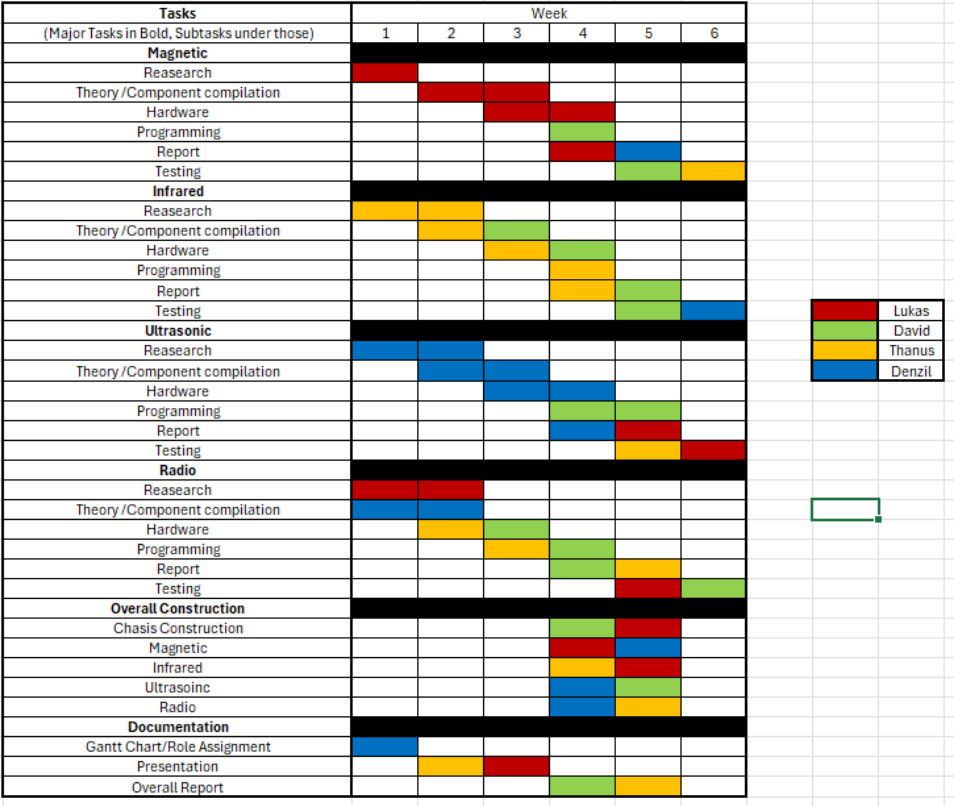
\includegraphics[width=0.8\textwidth]{subpages/images/gantt_chart.png}
    \caption{Gantt Chart}
    \label{fig:gantt}
\end{figure}

Key things to note from this Gantt chart and the subsequent planning include:
\begin{itemize}
    \item The `Overall Construction' main task and `Testing' subtasks were purposely handled by two people each in which those selected hadn’t done the other task for that specific part of the project (i.e. two people constructing the magnet circuit wouldn’t be responsible for testing the circuit). This was done to remove any potential bias, whether deliberate or otherwise.
    \item This chart was the final edition as if tasks, when practically worked on, were deemed as trivial, this would give members in the group spare time allowing for further collaboration in the more time-consuming subtasks of the project.
    \item Most importantly, this plan does not restrict members of the team moving and assisting other members with their construction or testing. Though, this should only be if they have made sufficient progress or completed their own section.
\end{itemize}